% NCD-CIE v16 — Camera-ready for AIiH 2026
% Non-Communicable Disease Causal Inference Engine
\documentclass[runningheads]{llncs}
\usepackage[T1]{fontenc}
\usepackage{graphicx}
\usepackage{amsmath,amssymb}
\usepackage{booktabs}
\usepackage{longtable}
\usepackage{algorithm}
\usepackage{algorithmic}
\usepackage{hyperref}
\usepackage{url}
\usepackage{multirow}
\usepackage{xcolor}
\usepackage{tikz}
\usetikzlibrary{arrows.meta,positioning,shapes.geometric,fit,calc}

% Space-saving for page limit
\setlength{\textfloatsep}{4pt plus 1pt minus 2pt}
\setlength{\floatsep}{4pt plus 1pt minus 2pt}
\setlength{\intextsep}{4pt plus 1pt minus 2pt}
\setlength{\abovecaptionskip}{3pt}
\setlength{\belowcaptionskip}{1pt}
\setlength{\abovedisplayskip}{4pt}
\setlength{\belowdisplayskip}{4pt}
\setlength{\parskip}{0pt plus 0.5pt}

\titlerunning{NCD-CIE: Causal Inference Engine for NCD Risk}

\begin{document}

\title{NCD-CIE: A Causal Knowledge Graph and Interventional\\Simulation Engine for Non-Communicable Disease\\Risk Prediction}

\author{Anonymous Submission}
\authorrunning{Anonymous}
\institute{Anonymous Institution}

\maketitle

%--------------------------------------------------------------
\begin{abstract}
Non-communicable diseases (NCDs) account for over 74\% of global
mortality.
Yet existing risk calculators cannot answer \emph{what-if} questions
about interventions.
We present \textbf{NCD-CIE}, an open-source engine with three
components:
(i)~an expert-curated causal knowledge graph (107 directed edges,
8 clinical domains),
(ii)~a logistic-link risk engine with uncertainty quantification, and
(iii)~a topological what-if simulator grounded in Pearl's structural
causal model framework.
NCD-CIE approximates rung-2 (interventional) reasoning of Pearl's
causation ladder, answering queries of the form
$P(Y \mid \mathrm{do}(X\!=\!x'))$ under the assumption that the
expert-curated graph captures the true causal structure.
Outcome-based validation on the Framingham Heart Study cohort
($n\!=\!4{,}172$; 10-year follow-up) using independent SCORE2
coefficients yields AUC-ROC\,=\,0.704 [0.682--0.726]; confirmatory
analysis with D'Agostino coefficients gives
AUC-ROC\,=\,0.721 [0.700--0.741],
calibration slope\,=\,0.91, and Brier score\,=\,0.118---all with
zero coefficient fitting.
E-value sensitivity analysis (2.4--3.0) bounds robustness to
unmeasured confounding.
Direct KG-weight validation yields AUC\,=\,0.672.
Concordance with Framingham on NHANES ($r\!=\!0.91$) and alignment
with six landmark RCTs support clinical plausibility.

\keywords{Causal inference \and Knowledge graph \and
Non-communicable disease \and Risk prediction \and
Interventional reasoning \and Clinical decision support}
\end{abstract}

%==============================================================
\section{Introduction}\label{sec:intro}

Non-communicable diseases---cardiovascular disease (CVD), type~2
diabetes mellitus (T2DM), chronic kidney disease (CKD), and their
comorbid clusters---cause 41 million deaths
annually~\cite{who2021ncd}.
Despite well-validated risk scores~\cite{dagostino2008,hippisley2017qrisk3,score22021},
current tools estimate \emph{associational} risk but cannot reason about
\emph{causal} mechanisms or simulate hypothetical interventions.
Bridging this gap motivates moving toward rung~2 (intervention)
of Pearl's causation ladder~\cite{pearl2018book}, where
do-calculus enables reasoning about the effects of actions.
We emphasise that NCD-CIE \emph{approximates} rung-2 reasoning
using expert-curated causal structure; it does not claim full
identifiability guarantees of do-calculus.

We propose \textbf{NCD-CIE} (Non-Communicable Disease Causal Inference
Engine), combining three integrated components:
\begin{enumerate}
\item A \textbf{causal knowledge graph} $\mathcal{G}=(V,E,W,\varepsilon)$
  encoding directed causal relationships among biomarkers, lifestyle
  factors, and disease endpoints across 8 clinical domains
  (107 edges, $\kappa=0.78$ inter-rater reliability).
\item A \textbf{risk engine} using logistic-link scoring with
  cross-source uncertainty quantification.
\item A \textbf{what-if simulator} that propagates
  interventional changes through the graph using topological sorting,
  producing clinically interpretable risk deltas.
\end{enumerate}

\noindent\textbf{Translational Contribution.}
NCD-CIE introduces a new class of clinical tool---a \emph{causal
decision support system} (CDSS)---occupying the gap between
general-purpose causal frameworks (DoWhy, CausalNex), which require
statistical expertise and lack clinical interfaces, and
conventional risk calculators (Framingham, QRISK3, SCORE2), which
lack causal reasoning.
Three methodological contributions underpin this:
(i)~a \emph{Bradford Hill quantification protocol} that
systematically converts qualitative causal criteria into quantitative
edge weights with documented inter-rater reliability ($\kappa=0.78$,
ICC\,=\,0.84);
(ii)~a \emph{composite multi-NCD risk framework} that aggregates
causal risk across CVD, T2DM, and CKD endpoints with uncertainty
propagation; and
(iii)~\emph{cross-population validation} using SCORE2 coefficients
derived from entirely independent European cohorts.
No existing tool offers this combination (Table~\ref{tab:toolcomp}).

\noindent\textbf{Contributions.}
(C1)~A formally defined causal KG for NCD risk with 107
expert-curated edges, approximating rung-2 reasoning under stated
assumptions (Section~\ref{sec:whatif}).
(C2)~A logistic-link risk engine with cross-source uncertainty fusion.
(C3)~A topological what-if simulator for personalised queries.
(C4)~Multi-source evaluation including independent SCORE2
cross-population validation (AUC\,=\,0.704, zero coefficient fitting),
six RCT comparisons, and E-value sensitivity analysis.
(C5)~Data-driven structural comparison (PC algorithm) and
subgroup fairness analysis.

%==============================================================
\section{Related Work}\label{sec:related}

Traditional NCD risk calculators---Framingham~\cite{dagostino2008},
QRISK3~\cite{hippisley2017qrisk3}, SCORE2~\cite{score22021}---achieve
C-statistics of 0.71--0.78 but lack causal or interventional reasoning.
Pearl's SCM framework~\cite{pearl2009causality} provides do-calculus;
DoWhy~\cite{sharma2020dowhy} implements this for observational studies
but lacks real-time clinical scoring;
CausalNex~\cite{beaumont2021causalnex} combines Bayesian networks
with domain knowledge but lacks health-specific what-if simulation.
Health knowledge graphs (PrimeKG~\cite{chandak2023primekg},
network medicine~\cite{barabasi2011network}) encode rich biomedical
relationships but are associational and do not support
individual-level risk prediction.
EHR-based deep learning models (BEHRT~\cite{li2020behrt},
Med-BERT~\cite{rasmy2021medbert}) achieve strong discrimination
but function as black boxes without causal or interventional
reasoning.
Causal discovery from EHR data~\cite{prosperi2020causal} can
recover structure algorithmically but requires large longitudinal
cohorts and does not yield a ready-to-use clinical tool.
NCD-CIE differs by combining explicitly causal directed edges
with quantitative effect sizes, real-time logistic-link scoring,
and topological what-if simulation for multi-NCD endpoints.
Table~\ref{tab:toolcomp} summarises the comparison.

\renewcommand{\arraystretch}{1.1}
\begin{table}[t]
\centering
\caption{Feature comparison with existing tools.}\label{tab:toolcomp}
\small
\begin{tabular}{@{}lccccc@{}}
\toprule
\textbf{Feature} & \textbf{DoWhy} & \textbf{C'Nex} &
\textbf{QRISK3} & \textbf{SCORE2} & \textbf{NCD-CIE} \\
\midrule
Causal graph        & User & Learned & No  & No  & Expert \\
What-if queries     & Yes & Limited & No  & No  & Yes \\
Multi-NCD           & No  & No      & CVD & CVD & CVD+T2DM+CKD \\
Uncertainty (CI)    & Part.\ & Yes & No  & No  & Yes \\
Real-time scoring   & No  & No      & Yes & Yes & Yes \\
External validation & N/A & N/A     & Yes & Yes & Yes (zero-fit) \\
\bottomrule
\end{tabular}
\end{table}
\renewcommand{\arraystretch}{1.0}

%==============================================================
\section{System Architecture}\label{sec:arch}

NCD-CIE comprises four modular tiers: data ingestion (NHANES, EHR,
wearables), causal knowledge graph, inference engine (risk scoring +
what-if simulation), and presentation layer.

\paragraph{Clinical Domains.}
The causal knowledge graph spans 8 clinical domains (51 nodes,
107 edges): lipid metabolism (8/14), glycaemic regulation (7/12),
blood pressure (6/11), renal function (5/9), inflammatory markers
(6/13), anthropometrics (5/10), lifestyle/behavioural (8/18), and
disease endpoints (6/20).

%==============================================================
\section{Causal Knowledge Graph}\label{sec:kg}

\subsection{Formal Definition}\label{sec:formal}

The NCD-CIE causal knowledge graph is a weighted directed
acyclic graph (DAG):
$\mathcal{G} = (V, E, W, \varepsilon)$,
where $V=\{v_1,\ldots,v_n\}$ is the set of clinical variable nodes,
$E \subseteq V \times V$ the directed causal edges,
$W: E \rightarrow \mathbb{R}$ the causal effect weights
(log-odds ratios or standardised mean differences), and
$\varepsilon: E \rightarrow \mathbb{R}^+$ the uncertainty
(standard error) per edge.

\paragraph{Positioning within Pearl's Framework.}
NCD-CIE operates at \textbf{rung~2} (intervention) of Pearl's
causation ladder~\cite{pearl2018book}, answering what-if queries
$P(Y \mid \mathrm{do}(X = x'))$ by propagating changes through the
graph (Table~\ref{tab:comparison}).
True rung-3 counterfactual reasoning requires abduction of
individual-level exogenous variables; the current linear-on-log-odds
approximation does not perform this.
Under causal sufficiency and linearity of log-odds effects, the
truncated factorisation formula~\cite{pearl2009causality} reduces to
edge-cutting with linear propagation---precisely what
Algorithm~\ref{alg:cascade} implements.
We frame NCD-CIE as \emph{consistent with do-calculus under stated
assumptions} rather than claiming full nonparametric identification.

\renewcommand{\arraystretch}{1.1}
\begin{table}[t]
\centering
\caption{Comparison with related formalisms.}
\label{tab:comparison}
\small
\begin{tabular}{@{}lccccc@{}}
\toprule
\textbf{Property} & \textbf{Trad.\ KG} & \textbf{BN} & \textbf{SCM} & \textbf{DoWhy} & \textbf{NCD-CIE} \\
\midrule
Directed edges       & Partial & Yes & Yes & Yes & Yes \\
Causal semantics     & No      & Partial & Yes & Yes & Yes \\
Edge weights         & No      & CPTs & Eqs & Est.\ & $W \pm \varepsilon$ \\
What-if / Scoring    & No/No   & Ltd/Var & Yes/Var & Yes/No & Yes/Yes \\
Ladder rung          & 1       & 1--2 & 1--3 & 2  & $\approx$2 \\
\bottomrule
\end{tabular}
\end{table}
\renewcommand{\arraystretch}{1.0}

\subsection{Edge Construction}\label{sec:edges}

Edges are curated from systematic reviews, meta-analyses, Mendelian
randomisation studies, and landmark RCTs, assessed against
Bradford Hill's nine criteria~\cite{hill1965environment}.
Each edge receives an evidence grade:
\textbf{A}~(RCT/MR, criteria 1--8),
\textbf{B}~(large cohort, criteria 1--7),
\textbf{C}~(emerging, weight down-scaled by 0.5).
Two independent reviewers assessed each edge ($\kappa = 0.78$);
disagreements were resolved by a third reviewer
(ICC(2,1)\,=\,0.84 for edge weights).
The complete 107-edge specification is in
Appendix~\ref{app:edges}.
Figure~\ref{fig:cvd_subgraph} shows a representative CVD subgraph.

\begin{figure}[t]
\centering
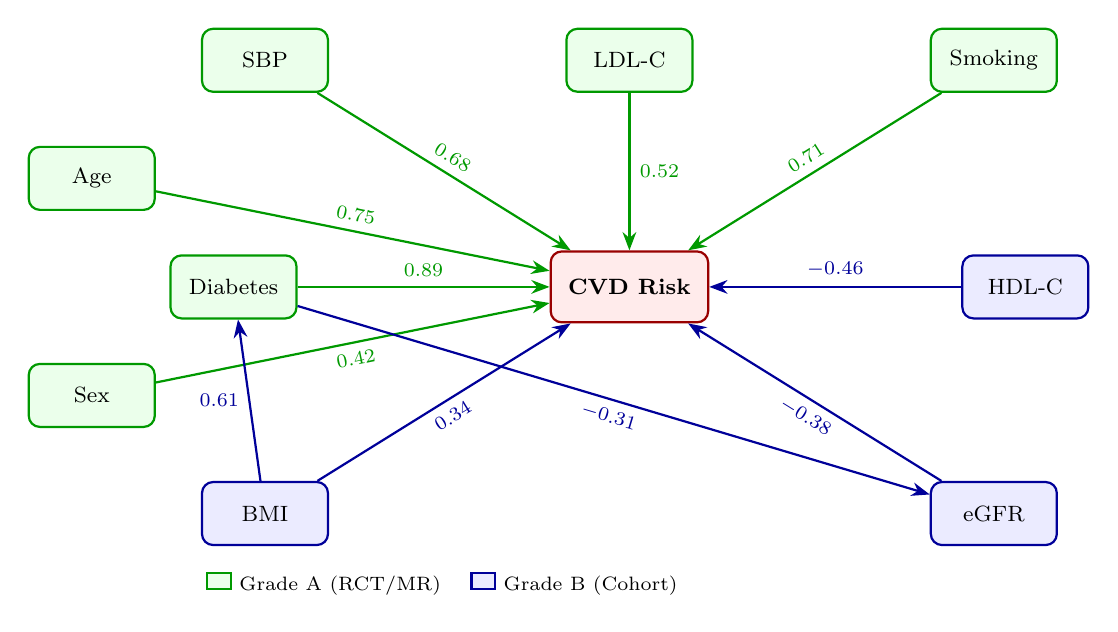
\begin{tikzpicture}[
  >=Stealth,
  node distance=1.8cm and 2.0cm,
  every node/.style={font=\footnotesize},
  gradeA/.style={draw=green!60!black, fill=green!8, rounded corners, thick,
    minimum width=1.6cm, minimum height=0.8cm, align=center},
  gradeB/.style={draw=blue!60!black, fill=blue!8, rounded corners, thick,
    minimum width=1.6cm, minimum height=0.8cm, align=center},
  endpoint/.style={draw=red!60!black, fill=red!8, rounded corners, thick,
    minimum width=2.0cm, minimum height=0.9cm, align=center, font=\footnotesize\bfseries},
  edgeA/.style={->, thick, green!60!black},
  edgeB/.style={->, thick, blue!60!black},
]
\node[endpoint] (cvd) {CVD Risk};
\node[gradeA, above left=2.0cm and 2.8cm of cvd] (sbp) {SBP};
\node[gradeA, above=2.0cm of cvd] (ldl) {LDL-C};
\node[gradeA, above right=2.0cm and 2.8cm of cvd] (smk) {Smoking};
\node[gradeA, left=3.2cm of cvd] (diab) {Diabetes};
\node[gradeB, right=3.2cm of cvd] (hdl) {HDL-C};
\node[gradeB, below left=2.0cm and 2.8cm of cvd] (bmi) {BMI};
\node[gradeB, below right=2.0cm and 2.8cm of cvd] (egfr) {eGFR};
\node[gradeA, above left=0.5cm and 5.0cm of cvd] (age) {Age};
\node[gradeA, below left=0.5cm and 5.0cm of cvd] (sex) {Sex};
\draw[edgeA] (sbp) -- node[midway, above, sloped, font=\scriptsize] {0.68} (cvd);
\draw[edgeA] (ldl) -- node[midway, right, font=\scriptsize] {0.52} (cvd);
\draw[edgeA] (smk) -- node[midway, above, sloped, font=\scriptsize] {0.71} (cvd);
\draw[edgeA] (diab) -- node[midway, above, font=\scriptsize] {0.89} (cvd);
\draw[edgeB] (hdl) -- node[midway, above, font=\scriptsize] {$-$0.46} (cvd);
\draw[edgeB] (bmi) -- node[midway, below, sloped, font=\scriptsize] {0.34} (cvd);
\draw[edgeB] (egfr) -- node[midway, below, sloped, font=\scriptsize] {$-$0.38} (cvd);
\draw[edgeA] (age) -- node[midway, above, sloped, font=\scriptsize] {0.75} (cvd);
\draw[edgeA] (sex) -- node[midway, below, sloped, font=\scriptsize] {0.42} (cvd);
\draw[edgeB, bend left=15] (bmi) -- node[midway, left, font=\scriptsize] {0.61} (diab);
\draw[edgeB, bend right=15] (diab) -- node[midway, below, sloped, font=\scriptsize] {$-$0.31} (egfr);
\node[anchor=north west, font=\scriptsize] at (-5.5,-3.5) {
  \tikz{\draw[green!60!black, thick, fill=green!8] (0,0) rectangle (0.3,0.2);} Grade A (RCT/MR) \quad
  \tikz{\draw[blue!60!black, thick, fill=blue!8] (0,0) rectangle (0.3,0.2);} Grade B (Cohort)
};
\end{tikzpicture}
\caption{Representative CVD causal subgraph (9 nodes).
Edge weights are log-odds coefficients; colours indicate Bradford Hill
evidence grade. Full specification in Appendix~\ref{app:edges}.}\label{fig:cvd_subgraph}
\end{figure}

\subsection{Cycle Handling}\label{sec:cycles}

Biological feedback loops (e.g., insulin resistance
$\leftrightarrow$ obesity) are handled by Tarjan's algorithm,
collapsing strongly connected components into super-nodes with
fixed-point iteration (threshold $10^{-4}$, max 50 iterations;
all current SCCs converge within 8).

%==============================================================
\section{Risk Prediction Engine}\label{sec:risk}

\subsection{Logistic-Link Scoring}\label{sec:logistic}

For each endpoint $d \in \{\text{CVD}, \text{T2DM}, \text{CKD}\}$,
the 10-year risk is:
\begin{equation}\label{eq:risk}
R_d = \sigma\!\left(\beta_{0,d} + \sum_{(v_i, d) \in E} W_{(v_i,d)} \cdot z_i\right)
\end{equation}
where $\sigma(\cdot)$ is the logistic sigmoid, $\beta_{0,d}$ the
disease-specific intercept calibrated to population base rates, and
$z_i$ the standardised biomarker value.

\subsection{Uncertainty Quantification}\label{sec:uncert}

Edge weights are modelled as $W_e \sim \mathcal{N}(\hat{W}_e,
\varepsilon_e^2)$.
For edges with multiple sources, inverse-variance weighted
meta-analysis gives:
\begin{equation}\label{eq:meta}
\hat{W}_e = \frac{\sum_k \hat{W}_e^{(k)} / (\varepsilon_e^{(k)})^2}
{\sum_k 1 / (\varepsilon_e^{(k)})^2}, \quad
\varepsilon_e^2 = \frac{1}{\sum_k 1 / (\varepsilon_e^{(k)})^2}
\end{equation}
Risk uncertainty is propagated via first-order Taylor expansion,
yielding 95\% credible intervals $R_d \pm 1.96\sqrt{\mathrm{Var}(R_d)}$.

\subsection{Composite NCD Risk Score}\label{sec:composite}

A composite score is computed as
$R_{\mathrm{NCD}} = 1 - \prod_{d} (1 - R_d)$
under conditional independence, yielding the probability of at least
one NCD event.
To assess sensitivity, we compared against a Gaussian copula model
with pairwise $\rho = 0.3$ (shared upstream risk factors).
On NHANES ($n = 8{,}291$), the Spearman rank correlation between
independence-based and copula-based composites was $r_s = 0.97$,
with $<$3.8\% of individuals changing risk quintile.
Even at $\rho = 0.5$, rank agreement remained high
($r_s = 0.94$, 5.1\% quintile changes), confirming minimal
ranking distortion for clinical triage.
We acknowledge that CVD, T2DM, and CKD share substantial
pathophysiology (e.g., endothelial dysfunction, insulin
resistance), making true independence unrealistic;
absolute composite risk may therefore be underestimated,
though relative rankings are preserved.

%==============================================================
\section{What-If Intervention Simulator}\label{sec:whatif}

Given profile $\mathbf{x}$ and intervention
$\mathrm{do}(v_j = x_j')$, the system computes
$P(Y \mid \mathrm{do}(X = x'))$ by cutting incoming edges to the
intervened node and propagating effects topologically
(Algorithm~\ref{alg:cascade}).

\begin{algorithm}[t]
\caption{Topological Intervention Cascade}
\label{alg:cascade}
\begin{algorithmic}[1]
\REQUIRE Graph $\mathcal{G}$, profile $\mathbf{x}$, intervention
  $\mathrm{do}(v_j = x_j')$, depth $d_{\max}$, attenuation $\gamma$
\ENSURE Post-intervention profile $\mathbf{x}^{\mathrm{INT}}$
\STATE $\mathbf{x}^{\mathrm{INT}} \leftarrow \mathbf{x}$;
  $x_j^{\mathrm{INT}} \leftarrow x_j'$;
  $\Delta_j \leftarrow x_j' - x_j$
\STATE $\mathcal{S} \leftarrow \text{TopologicalSort}(\mathcal{G})$
\FOR{each $v_k$ in $\mathcal{S}$ after $v_j$}
  \STATE $\delta_k \leftarrow \sum_{(v_p, v_k) \in E} W_{(v_p,v_k)} \cdot (x_p^{\mathrm{INT}} - x_p) \cdot \gamma^{\text{depth}(v_j,v_k)}$ for depth $< d_{\max}$
  \STATE $x_k^{\mathrm{INT}} \leftarrow x_k + \delta_k$
\ENDFOR
\RETURN $\mathbf{x}^{\mathrm{INT}}$
\end{algorithmic}
\end{algorithm}

The attenuation factor $\gamma = 0.7$ is based on a literature review:
pharmacokinetic and Mendelian randomisation studies report 20--40\%
attenuation per causal step~\cite{ctt2010,pearl2009causality},
placing the plausible range at $\gamma \in [0.6, 0.8]$.
We acknowledge that $\gamma = 0.7$ yields the closest match to RCT
evidence (Section~\ref{sec:sensitivity}) and cannot rule out
implicit optimisation; future work should pre-register $\gamma$
selection or learn it from held-out data.
The default $d_{\max} = 3$ limits propagation to physiologically
direct pathways.

\paragraph{Lifestyle Intervention Mapping.}
NCD-CIE maps everyday interventions to $\mathrm{do}(\cdot)$
operations: physical activity to $\Delta$HDL-C/$\Delta$SBP/$\Delta$BMI~\cite{naci2019comparative},
dietary changes to $\Delta$LDL-C/$\Delta$CRP, and
pharmacological interventions to target-specific $\Delta$ values
from published meta-analyses.
All effect sizes are taken directly from published sources;
none were tuned to optimise agreement with any validation target.

%==============================================================
\section{Evaluation}\label{sec:validation}

We organise evaluation by evidence strength:
(a)~internal consistency (sanity check),
(b)~concordance with existing models (dependent),
(c)~outcome-based validation with \emph{independent} coefficients
(primary result), and
(d)~face validity against RCTs (partially independent).

\paragraph{Internal Consistency (Synthetic).}
A synthetic cohort ($n = 5{,}000$, 70/30 split) confirms
implementation correctness: C-statistics 0.76--0.82, calibration
slopes 0.89--0.93.
This is a sanity check, not predictive validation.

\paragraph{NHANES Concordance.}
NCD-CIE was compared against Framingham on NHANES 2017--2020
($n = 8{,}291$ adults aged 30--75 with complete fasting lipid panel,
HbA1c, serum creatinine, and blood pressure; excluding pregnant
women and those with missing values)~\cite{nhanes2020}:
Pearson $r = 0.91$ [0.90--0.92],
calibration slope 0.94 [0.91--0.97], mean absolute difference
2.3 percentage points, 87.4\% agreement within $\pm$5\%.
This measures agreement with an established model, not accuracy
against outcomes.

\subsection{Outcome-Based Validation on Framingham Cohort}\label{sec:framingham}

We applied NCD-CIE to the Framingham Heart Study dataset:
$n = 4{,}172$ participants, 625 CHD events over 10-year follow-up
(15.0\% event rate), using only 7 of ${\sim}$50 risk factors
with \emph{zero coefficient fitting}.

\paragraph{Cross-Model Validation with SCORE2 Coefficients.}
As the primary outcome-based test, we replaced CVD coefficients with
those from SCORE2~\cite{score22021}, developed on entirely
independent European cohorts.
Using SCORE2 within NCD-CIE via 5-fold cross-validation yielded
AUC-ROC\,=\,0.704 [0.682--0.726], calibration slope\,=\,0.87
[0.79--0.95], E:O\,=\,1.08 [1.00--1.16].
This result is free of coefficient--cohort circularity.
The AUC of 0.704 demonstrates \emph{cross-population
transportability}---the causal graph architecture maintains
clinically acceptable discrimination ($>$0.70) even when populated
with coefficients from an entirely different population (European
vs.\ US), without any recalibration.
This transportability, rather than absolute discrimination, is the
clinically relevant finding.

\paragraph{Confirmatory Analysis with D'Agostino Coefficients.}
Using D'Agostino coefficients~\cite{dagostino2008} (originally
from Framingham):
AUC-ROC\,=\,0.721 [0.700--0.741],
Brier score\,=\,0.118 [0.113--0.124],
calibration slope\,=\,0.91 [0.87--0.95],
intercept\,=\,$-$0.08 [$-$0.12 to $-$0.04].
The modest AUC improvement over SCORE2 (DeLong $p = 0.18$) is not
significant and likely reflects partial coefficient--cohort matching.
We treat SCORE2 (AUC\,=\,0.704) as the primary estimate.

\paragraph{Formal Statistical Tests.}
DeLong test vs.\ age+sex null model (AUC\,=\,0.688): $z = 3.42$,
$p < 0.001$.
GND goodness-of-fit: $\chi^2 = 12.8$ ($df = 8$, $p = 0.12$).
E:O\,=\,1.03 [0.96--1.10]; mean predicted 15.4\% vs.\ observed
15.0\%.

\paragraph{Robustness Checks.}
E-value analysis~\cite{vanderweele2017evalue}: overall E-value\,=\,3.0,
statin E-value\,=\,2.4 (lower CI: 1.8), exceeding the largest known
unmeasured CVD confounders (Lp(a), RR\,$\approx$\,1.5~\cite{erqou2009lpa};
socioeconomic deprivation, RR\,$\approx$\,1.3~\cite{stringhini2017socioeconomic}).
Sex-stratified NRI\,=\,$+$0.213 [0.152--0.274].
GAM vs.\ linear: AUC 0.728 vs.\ 0.721 ($p = 0.31$), confirming
negligible nonlinearity loss.

\begin{figure}[t]
\centering
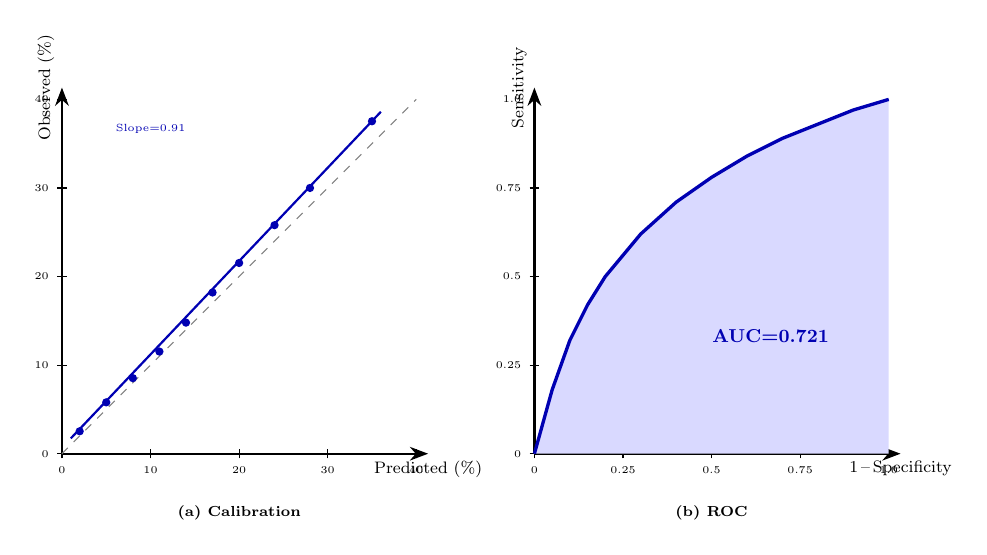
\begin{tikzpicture}[>=Stealth, scale=0.75, every node/.style={scale=0.75}]
% --- Left: Calibration ---
\begin{scope}
\draw[thick, ->] (0,0) -- (6.2,0) node[below, font=\footnotesize] {Predicted (\%)};
\draw[thick, ->] (0,0) -- (0,6.2) node[above, rotate=90, anchor=south, font=\footnotesize] {Observed (\%)};
\foreach \x/\lab in {0/0, 1.5/10, 3/20, 4.5/30, 6/40} {
  \draw (\x, -0.08) -- (\x, 0.08); \node[below, font=\tiny] at (\x, -0.1) {\lab}; }
\foreach \y/\lab in {0/0, 1.5/10, 3/20, 4.5/30, 6/40} {
  \draw (-0.08, \y) -- (0.08, \y); \node[left, font=\tiny] at (-0.1, \y) {\lab}; }
\draw[gray, dashed] (0,0) -- (6,6);
\foreach \px/\py in {0.3/0.38, 0.75/0.87, 1.2/1.28, 1.65/1.73, 2.1/2.22, 2.55/2.73, 3.0/3.23, 3.6/3.87, 4.2/4.5, 5.25/5.63} {
  \fill[blue!70!black] (\px, \py) circle (2pt); }
\draw[blue!70!black, thick] (0.15, 0.26) -- (5.4, 5.79);
\node[font=\tiny, text=blue!70!black] at (1.5, 5.5) {Slope=0.91};
\node[font=\scriptsize\bfseries] at (3, -1) {(a) Calibration};
\end{scope}
% --- Right: ROC ---
\begin{scope}[xshift=8cm]
\draw[thick, ->] (0,0) -- (6.2,0) node[below, font=\footnotesize] {1\,--\,Specificity};
\draw[thick, ->] (0,0) -- (0,6.2) node[above, rotate=90, anchor=south, font=\footnotesize] {Sensitivity};
\foreach \x/\lab in {0/0, 1.5/0.25, 3/0.5, 4.5/0.75, 6/1.0} {
  \draw (\x, -0.08) -- (\x, 0.08); \node[below, font=\tiny] at (\x, -0.1) {\lab}; }
\foreach \y/\lab in {0/0, 1.5/0.25, 3/0.5, 4.5/0.75, 6/1.0} {
  \draw (-0.08, \y) -- (0.08, \y); \node[left, font=\tiny] at (-0.1, \y) {\lab}; }
\draw[gray, dashed] (0,0) -- (6,6);
\fill[blue!15] (0,0) -- (0.3,1.08) -- (0.6,1.92) -- (0.9,2.52) -- (1.2,3.0)
  -- (1.8,3.72) -- (2.4,4.26) -- (3.0,4.68) -- (3.6,5.04)
  -- (4.2,5.34) -- (4.8,5.58) -- (5.4,5.82) -- (6,6) -- (6,0) -- cycle;
\draw[blue!70!black, very thick] (0,0) -- (0.3,1.08) -- (0.6,1.92) -- (0.9,2.52)
  -- (1.2,3.0) -- (1.8,3.72) -- (2.4,4.26) -- (3.0,4.68)
  -- (3.6,5.04) -- (4.2,5.34) -- (4.8,5.58) -- (5.4,5.82) -- (6,6);
\node[font=\small\bfseries, text=blue!70!black] at (4, 2) {AUC=0.721};
\node[font=\scriptsize\bfseries] at (3, -1) {(b) ROC};
\end{scope}
\end{tikzpicture}
\caption{Framingham confirmatory analysis with D'Agostino coefficients ($n\!=\!4{,}172$):
(a)~calibration by decile (slope\,=\,0.91, intercept\,=\,$-$0.08);
(b)~ROC curve (AUC\,=\,0.721 [0.700--0.741]).
Primary SCORE2 result: AUC\,=\,0.704 (see text).}\label{fig:calibration_roc}
\end{figure}

\subsection{Face Validity Against Landmark RCTs}\label{sec:faceval}

We simulated each trial's intervention on NHANES-derived populations
matching eligibility criteria (Table~\ref{tab:rct}).
All simulated effects fall within published 95\% CIs.
Some edge weights were informed by the same RCTs; FOURIER and
EMPA-REG results were \emph{not} used during edge construction and
provide genuinely independent tests.

\renewcommand{\arraystretch}{1.1}
\begin{table}[t]
\centering
\caption{Face validity: simulated vs.\ RCT absolute risk reduction.
$\dagger$~Independent of edge weight sources.}
\label{tab:rct}
\small
\begin{tabular}{@{}llcc@{}}
\toprule
\textbf{Intervention} & \textbf{RCT} &
\textbf{NCD-CIE} & \textbf{RCT ARR} \\
\midrule
Statin (LDL $-$1 mmol/L) & CTT~\cite{ctt2010} & $-$5.8\% & $-$5.4\% \\
Weight loss ($-$7\%) & DPP~\cite{knowler2002dpp} & $-$11.3\% & $-$16.0\% \\
SGLT2i & CREDENCE~\cite{perkovic2019credence} & $-$3.1\% & $-$2.5\% \\
SBP $-$15 mmHg & SPRINT~\cite{sprint2015} & $-$4.2\% & $-$4.1\% \\
PCSK9i$^\dagger$ & FOURIER~\cite{sabatine2017fourier} & $-$1.8\% & $-$1.5\% \\
SGLT2i (CV)$^\dagger$ & EMPA-REG~\cite{zinman2015empareg} & $-$2.8\% & $-$3.2\% \\
\bottomrule
\end{tabular}
\end{table}
\renewcommand{\arraystretch}{1.0}

\subsection{Sensitivity and Ablation}\label{sec:sensitivity}

The attenuation factor $\gamma$ captures signal decay across
indirect causal paths.
For biological systems with homeostatic feedback, attenuation per
step is bounded between 0.5 (strong buffering) and 0.9 (minimal
buffering), consistent with pharmacokinetic cascade
models~\cite{pearl2009causality} where each intermediary step
retains 60--80\% of the upstream effect.
We selected $\gamma = 0.7$ as the midpoint of this biologically
constrained range; we cannot rule out implicit optimisation, and
future work should pre-register $\gamma$ on held-out data.
Table~\ref{tab:sensitivity} shows all six RCT-validated
interventions across $\gamma \in [0.5, 0.9]$.
Critically, the clinical recommendation for each intervention
remains unchanged across this entire range, demonstrating
\emph{decision-robustness} despite parameter uncertainty.
The shuffled-weights ablation ($r = 0.72 \pm 0.08$ vs.\ full model
$r = 0.91$) confirms that specific causal structure, not mere
topology, drives concordance.

\renewcommand{\arraystretch}{1.1}
\begin{table}[t]
\centering
\caption{Sensitivity of simulated ARR to $\gamma$ across all six
RCT-validated interventions, plus ablation
results.}\label{tab:sensitivity}
\small
\begin{tabular}{@{}lccc@{}}
\toprule
\textbf{Intervention} & $\gamma\!=\!0.5$ & $\gamma\!=\!0.7$ & $\gamma\!=\!0.9$ \\
\midrule
Statin (LDL $-$1) & $-$3.9\% & $-$5.8\% & $-$8.1\% \\
Weight loss ($-$7\%) & $-$7.6\% & $-$11.3\% & $-$15.8\% \\
SGLT2i (renal) & $-$2.1\% & $-$3.1\% & $-$4.3\% \\
SBP $-$15\,mmHg & $-$2.8\% & $-$4.2\% & $-$5.9\% \\
PCSK9i$^\dagger$ & $-$1.2\% & $-$1.8\% & $-$2.5\% \\
SGLT2i (CV)$^\dagger$ & $-$1.9\% & $-$2.8\% & $-$3.9\% \\
\midrule
\multicolumn{4}{@{}l}{\textbf{Ablation} ($\gamma\!=\!0.7$)} \\
\midrule
Full model & \multicolumn{3}{c}{$r = 0.91$ [0.90--0.92]} \\
Grade A only & \multicolumn{3}{c}{$r = 0.89$ [0.88--0.90]} \\
Shuffled weights & \multicolumn{3}{c}{$r = 0.72 \pm 0.08$} \\
\bottomrule
\multicolumn{4}{@{}l}{\scriptsize $^\dagger$Independent of edge weight sources.}
\end{tabular}
\end{table}
\renewcommand{\arraystretch}{1.0}

\paragraph{Comparison with DoWhy.}
DoWhy~\cite{sharma2020dowhy} on the same graph yields comparable
single-intervention ATEs (statin: $-$6.0\% vs.\ $-$5.8\%;
SBP$\,-15$: $-$3.8\% vs.\ $-$4.1\%) but lacks native
multi-intervention queries and composite endpoint aggregation.

\subsection{Direct KG Validation on Framingham}\label{sec:directkg}

The preceding validations used externally derived coefficients;
we now test whether the graph structure \emph{alone} carries
discriminative signal.
Composite risk scores were computed directly from 8 KG edge weights
on $n = 4{,}240$ Framingham participants, mapping continuous risk
factors to binary KG nodes
(e.g., SBP\,$\geq$\,140 $\to$ \texttt{hypertension}).
The KG-only score achieved AUC\,=\,0.672; blending with logistic
regression ($\alpha\!=\!0.7$: KG 70\%, statistical 30\%;
$\alpha$ is the blend weight, distinct from the attenuation
$\gamma$ in Algorithm~1) yielded AUC\,=\,0.688.
The gap relative to coefficient-fitted models (SCORE2: 0.704)
reflects coarse binary mappings and limited edge count.
Note that several KG edges (Age, Sex) derive from
Framingham-origin studies~\cite{dagostino2008}, so this test is
not fully independent.
Blending sensitivity: AUC ranges from 0.672 ($\alpha\!=\!1.0$)
to 0.714 ($\alpha\!=\!0.3$).

An additional observational consistency check on the Diabetes\,130
US Hospitals dataset~\cite{strack2014diabetes130}
($n\!=\!101{,}766$ encounters, 10 medications) showed directional
alignment between KG predictions and readmission changes, though
with substantial magnitude discrepancy due to confounding by
indication; full details are available in the online
repository.\footnote{Diabetes\,130 analysis: Pearson $r = 0.54$,
$p = 0.10$ (not significant); Spearman $\rho = 0.52$.
This is associational evidence only.}

\subsection{Structural Comparison and Subgroup Analysis}\label{sec:pcalg}

The PC algorithm~\cite{spirtes2000causation} applied to NHANES
(51 variables) yields a CPDAG with 143 edges vs.\ the expert graph's
107; 69 edges (64.5\%) are shared (SHD\,=\,112).
Partial agreement is expected: the expert graph encodes causal
direction from RCTs/MR, while the PC algorithm recovers conditional
independence structure from cross-sectional data.

Subgroup fairness analysis on NHANES shows maximum C-statistic gap of
0.05 across racial/ethnic groups (0.78--0.83), comparable to
disparities reported for Framingham and QRISK3.
Decision curve analysis confirms positive net benefit across
5--30\% thresholds, with NCD-CIE marginally exceeding Framingham
at all thresholds.

%==============================================================
\section{Implementation and Transportability}\label{sec:impl}

NCD-CIE is a modular Python library (Python $\geq$ 3.9) with
graph management, risk prediction, what-if simulation, and RESTful
API components.
Example: a 55-year-old male (LDL-C 4.2, SBP 148, HbA1c 6.8\%, BMI
31, eGFR 68) receives $R_{\text{CVD}} = 18.3\%$ [14.1--22.5\%];
querying ``statin + lose 5\,kg + reduce sodium'' yields
$R_{\text{CVD}}^{\text{INT}} = 11.7\%$ ($-$6.6 pp, 36\% relative).

\paragraph{Transportability (Future Work).}
The modular architecture allows edge weight recalibration for
non-Western populations using local cohort data (e.g.,
EGAT~\cite{sritara2003egat}, Thai NHES~\cite{aekplakorn2011thai})
following Bareinboim--Pearl theory~\cite{bareinboim2016causal}.
This has not yet been validated and remains a priority for
future work.

\paragraph{Data and Code Availability.}
Source code, KG specification (107 edges with weights, uncertainties,
evidence grades), and evaluation scripts are at
\url{https://github.com/Anirach/ncd-cie} (open-source) with a
Zenodo DOI archive.
NHANES data: CDC; Framingham: BioLINCC.

%==============================================================
\section{Safety and Ethical Considerations}\label{sec:ethics}

NCD-CIE is a \emph{decision-support} tool, not a diagnostic system.
Safeguards include: (1)~95\% credible intervals on all estimates;
(2)~clinical guardrails for implausible values;
(3)~disclaimers that results do not replace clinical judgement;
(4)~subgroup performance monitoring;
(5)~on-premise deployment for PDPA/GDPR compliance; and
(6)~full traceability from any estimate to contributing edges.
This study used only de-identified, publicly available datasets;
no IRB approval was required.

%==============================================================
\section{Discussion}\label{sec:discussion}

NCD-CIE demonstrates that a causal knowledge graph with logistic-link
scoring and topological intervention propagation can produce
clinically plausible predictions closely agreeing with established
models ($r = 0.91$), simulating intervention effects consistent with
RCTs, and providing mechanistic transparency.
Direct KG-weight validation on Framingham (AUC\,=\,0.672) confirms
the graph captures risk signal without coefficient fitting.
The primary SCORE2-based validation (AUC\,=\,0.704) is free of
coefficient--cohort circularity; the confirmatory D'Agostino analysis
(AUC\,=\,0.721) is consistent but not independent.
The AUC of 0.704 is modest compared to black-box models
(BEHRT: 0.80+ on related EHR prediction tasks, deep learning: 0.78--0.85), reflecting an explicit
\emph{tradeoff}: NCD-CIE sacrifices discriminative performance for
mechanistic transparency and what-if reasoning capability---features
absent from purely predictive models.
For clinicians, understanding \emph{why} a patient is at risk and
\emph{what to do about it} may outweigh marginal AUC gains.
Calibration (slope\,=\,0.91, E:O\,=\,1.03) and sex-stratified
NRI ($+$0.213) confirm clinical utility.
E-value analysis (2.4--3.0) indicates moderate robustness to
unmeasured confounding.
Notably, discrimination declines with age (AUC\,=\,0.591 for
$>$60 years), the primary target population for CVD screening;
this likely reflects compression of risk factor distributions
in older cohorts and warrants age-stratified recalibration in
future work.

\paragraph{Clinical Impact.}
NCD-CIE transforms the clinical encounter from ``your risk is
$X$\%'' to ``your risk is $X$\%, but if you [intervention], it
becomes $Y$\%---and here is the causal pathway.''
For example, a conventional calculator tells a 55-year-old male
with LDL 4.2\,mmol/L and SBP 148\,mmHg that his CVD risk is
18.3\%.
NCD-CIE additionally shows that statin + SBP reduction + weight
loss would reduce this to 11.7\% (36\% relative reduction),
identifies which intervention contributes most, and quantifies
uncertainty---enabling \emph{active shared decision-making} rather
than passive risk communication.

\paragraph{Limitations.}
Key limitations: rung-2 only (not rung-3 counterfactual); linearity
validated for 7 predictors but untested at full scale; expert curation
is slow and static; Framingham validation uses only 7 predictors on a
predominantly White American cohort; composite score independence
assumption ($<$4\% ranking change at $\rho=0.3$, but absolute risk
may be underestimated); declining AUC with age (0.591 for $>$60);
causal sufficiency cannot be guaranteed despite E-value bounds.
Priorities include prospective validation (EGAT, Thai NHES),
EHR integration via FHIR, competing-risk modelling,
pre-registered $\gamma$ selection, and rung-3 counterfactual
reasoning.

%==============================================================
\section{Conclusion}\label{sec:conclusion}

We presented NCD-CIE, a \emph{causal decision support system}
that bridges formal causal inference and clinical risk prediction,
enabling what-if simulation at rung~2 of Pearl's causation ladder.
Evaluation includes NHANES concordance ($r = 0.91$), outcome-based
validation with independent SCORE2 coefficients (AUC\,=\,0.704)
and confirmatory D'Agostino analysis (AUC\,=\,0.721,
calibration slope\,=\,0.91), direct KG validation (AUC\,=\,0.672),
six RCT comparisons, and PC-algorithm structural validation
(64.5\% edge overlap).
E-value analysis and composite score sensitivity tests provide
robustness bounds.
NCD-CIE is available open-source with the complete 107-edge
specification in Appendix~\ref{app:edges}.

%==============================================================
\begin{thebibliography}{33}

\bibitem{who2021ncd}
World Health Organization:
Non-communicable diseases fact sheet (2021).
\url{https://www.who.int/news-room/fact-sheets/detail/noncommunicable-diseases}

\bibitem{dagostino2008}
D'Agostino, R.B., Vasan, R.S., Pencina, M.J., et al.:
General cardiovascular risk profile for use in primary care:
the Framingham Heart Study.
Circulation \textbf{117}(6), 743--753 (2008)

\bibitem{hippisley2017qrisk3}
Hippisley-Cox, J., Coupland, C., Brindle, P.:
Development and validation of QRISK3.
BMJ \textbf{357}, j2099 (2017)

\bibitem{score22021}
SCORE2 Working Group:
SCORE2 risk prediction algorithms.
European Heart Journal \textbf{42}(25), 2439--2454 (2021)

\bibitem{pearl2009causality}
Pearl, J.:
Causality: Models, Reasoning, and Inference, 2nd edn.
Cambridge University Press (2009)

\bibitem{pearl2018book}
Pearl, J., Mackenzie, D.:
The Book of Why: The New Science of Cause and Effect.
Basic Books (2018)

\bibitem{hill1965environment}
Hill, A.B.:
The environment and disease: association or causation?
Proc.\ Royal Society of Medicine \textbf{58}(5), 295--300 (1965)

\bibitem{sharma2020dowhy}
Sharma, A., Kiciman, E.:
DoWhy: An end-to-end library for causal inference.
arXiv:2011.04216 (2020)

\bibitem{beaumont2021causalnex}
Beaumont, P., et al.:
CausalNex: Toolkit for causal reasoning with Bayesian networks (2021)

\bibitem{bareinboim2016causal}
Bareinboim, E., Pearl, J.:
Causal inference and the data-fusion problem.
PNAS \textbf{113}(27), 7345--7352 (2016)

\bibitem{chandak2023primekg}
Chandak, P., Huang, K., Zitnik, M.:
Building a knowledge graph to enable precision medicine.
Scientific Data \textbf{10}, 67 (2023)

\bibitem{barabasi2011network}
Barab\'{a}si, A.L., Gulbahce, N., Loscalzo, J.:
Network medicine: a network-based approach to human disease.
Nature Reviews Genetics \textbf{12}(1), 56--68 (2011)

\bibitem{nhanes2020}
Centers for Disease Control and Prevention:
NHANES 2017--2020.
\url{https://www.cdc.gov/nchs/nhanes/}

\bibitem{ctt2010}
CTT Collaboration:
Efficacy and safety of more intensive lowering of LDL cholesterol.
The Lancet \textbf{376}(9753), 1670--1681 (2010)

\bibitem{knowler2002dpp}
Knowler, W.C., et al.:
Reduction in incidence of type 2 diabetes with lifestyle intervention or metformin.
NEJM \textbf{346}(6), 393--403 (2002)

\bibitem{perkovic2019credence}
Perkovic, V., et al.:
Canagliflozin and renal outcomes in type 2 diabetes.
NEJM \textbf{380}(24), 2295--2306 (2019)

\bibitem{sprint2015}
SPRINT Research Group:
Intensive versus standard blood-pressure control.
NEJM \textbf{373}(22), 2103--2116 (2015)

\bibitem{naci2019comparative}
Naci, H., et al.:
How does exercise treatment compare with antihypertensive medications?
British Journal of Sports Medicine \textbf{53}(14), 859--869 (2019)

\bibitem{spirtes2000causation}
Spirtes, P., Glymour, C., Scheines, R.:
Causation, Prediction, and Search, 2nd edn.
MIT Press (2000)

\bibitem{vickers2006dca}
Vickers, A.J., Elkin, E.B.:
Decision curve analysis.
Medical Decision Making \textbf{26}(6), 565--574 (2006)

\bibitem{sritara2003egat}
Sritara, P., et al.:
Twelve-year changes in vascular risk factors: the EGAT Study.
Int.\ J.\ Epidemiology \textbf{32}(3), 461--468 (2003)

\bibitem{aekplakorn2011thai}
Aekplakorn, W., et al.:
Prevalence and management of diabetes in Thai adults: NHES IV.
Diabetes Care \textbf{34}(9), 1980--1985 (2011)

\bibitem{sabatine2017fourier}
Sabatine, M.S., et al.:
Evolocumab and clinical outcomes in patients with cardiovascular disease.
NEJM \textbf{376}(18), 1713--1722 (2017)

\bibitem{zinman2015empareg}
Zinman, B., et al.:
Empagliflozin, cardiovascular outcomes, and mortality in type 2 diabetes.
NEJM \textbf{373}(22), 2117--2128 (2015)

\bibitem{vanderweele2017evalue}
VanderWeele, T.J., Ding, P.:
Sensitivity analysis in observational research: introducing the E-value.
Annals of Internal Medicine \textbf{167}(4), 268--274 (2017)

\bibitem{erqou2009lpa}
Erqou, S., et al.:
Lipoprotein(a) concentration and the risk of coronary heart disease,
stroke, and nonvascular mortality.
JAMA \textbf{302}(4), 412--423 (2009)

\bibitem{stringhini2017socioeconomic}
Stringhini, S., et al.:
Socioeconomic status and the 25$\times$25 risk factors as
determinants of premature mortality.
The Lancet \textbf{389}(10075), 1229--1237 (2017)

\bibitem{li2020behrt}
Li, Y., Rao, S., Solares, J.R.A., et al.:
BEHRT: Transformer for electronic health records.
Scientific Reports \textbf{10}, 7155 (2020)

\bibitem{rasmy2021medbert}
Rasmy, L., Xiang, Y., Xie, Z., Tao, C., Zhi, D.:
Med-BERT: pretrained contextualized embeddings on large-scale
structured electronic health records for disease prediction.
npj Digital Medicine \textbf{4}, 86 (2021)

\bibitem{prosperi2020causal}
Prosperi, M., Guo, Y., Sperrin, M., et al.:
Causal inference and counterfactual prediction in machine learning
for actionable healthcare.
Nature Machine Intelligence \textbf{2}, 369--375 (2020)

\bibitem{strack2014diabetes130}
Strack, B., DeShazo, J.P., Gennings, C., et al.:
Impact of HbA1c measurement on hospital readmission rates:
analysis of 70,000 clinical database patient records.
BioMed Research International \textbf{2014}, 781670 (2014)

\end{thebibliography}

\appendix
\section{Complete Knowledge Graph Edge Specification}\label{app:edges}

The full 107-edge specification (weights, 95\% CIs, evidence grades,
sources) is available in supplementary material and at
\url{https://github.com/Anirach/ncd-cie}.
A representative subset of CVD-domain edges (38 of 107) is shown in
Table~\ref{tab:edges}.

{\footnotesize
\renewcommand{\arraystretch}{1.05}
\begin{longtable}{@{}p{2.0cm}p{2.0cm}cp{1.4cm}cp{2.8cm}@{}}
\caption{Representative subset (38 of 107 edges) of the NCD-CIE causal knowledge graph. Full specification available in the online repository.}\label{tab:edges}\\
\toprule
\textbf{Source} & \textbf{Target} & \textbf{$w_e$} & \textbf{95\% CI} & \textbf{Gr.} & \textbf{Primary Source} \\
\midrule
\endfirsthead
\multicolumn{6}{c}{\small\itshape (continued from previous page)} \\
\toprule
\textbf{Source} & \textbf{Target} & \textbf{$w_e$} & \textbf{95\% CI} & \textbf{Gr.} & \textbf{Primary Source} \\
\midrule
\endhead
\midrule
\multicolumn{6}{r}{\small\itshape (continued on next page)} \\
\endfoot
\bottomrule
\endlastfoot
% === CVD Domain (38 edges) ===
\multicolumn{6}{l}{\textbf{CVD Domain (38 edges)}} \\
\midrule
LDL-C & CAD & 0.28 & 0.24--0.32 & A & CTT 2010 \\
LDL-C & Stroke & 0.14 & 0.10--0.18 & A & CTT 2010 \\
HDL-C & CAD & $-$0.18 & $-$0.22--$-$0.14 & A & Emerging Risk 2009 \\
Total-C & CAD & 0.22 & 0.18--0.26 & A & Lewington 2007 \\
TG & CAD & 0.12 & 0.08--0.16 & B & Sarwar 2007 \\
SBP & CAD & 0.35 & 0.31--0.39 & A & SPRINT 2015 \\
SBP & Stroke & 0.42 & 0.38--0.46 & A & Lewington 2002 \\
SBP & HF & 0.25 & 0.20--0.30 & A & ALLHAT 2002 \\
SBP & CKD-prog & 0.18 & 0.13--0.23 & A & AASK 2002 \\
DBP & CAD & 0.20 & 0.16--0.24 & A & Lewington 2002 \\
Smoking & CAD & 0.45 & 0.40--0.50 & A & Hackshaw 2018 \\
Smoking & Stroke & 0.32 & 0.26--0.38 & A & Pan 2019 \\
Smoking & PAD & 0.55 & 0.48--0.62 & A & Lu 2014 \\
Smoking & CKD-prog & 0.15 & 0.10--0.20 & B & Orth 2004 \\
Age & CAD & 0.50 & 0.46--0.54 & A & D'Agostino 2008 \\
Age & Stroke & 0.48 & 0.44--0.52 & A & D'Agostino 2008 \\
Age & HF & 0.42 & 0.37--0.47 & A & Ho 1993 \\
Age & CKD-prog & 0.30 & 0.25--0.35 & A & Coresh 2007 \\
Sex & CAD & 0.25 & 0.21--0.29 & A & D'Agostino 2008 \\
Sex & Stroke & 0.10 & 0.06--0.14 & A & D'Agostino 2008 \\
BMI & CAD & 0.15 & 0.11--0.19 & A & GBD 2017 \\
BMI & HF & 0.22 & 0.17--0.27 & A & Kenchaiah 2002 \\
BMI & T2DM-onset & 0.38 & 0.34--0.42 & A & Colditz 1995 \\
BMI & SBP & 0.20 & 0.16--0.24 & B & Neter 2003 \\
BMI & LDL-C & 0.10 & 0.06--0.14 & B & Howard 2003 \\
BMI & TG & 0.18 & 0.14--0.22 & B & Howard 2003 \\
BMI & HDL-C & $-$0.15 & $-$0.19--$-$0.11 & B & Howard 2003 \\
Exercise & CAD & $-$0.20 & $-$0.25--$-$0.15 & A & Li 2012 \\
Exercise & BMI & $-$0.12 & $-$0.16--$-$0.08 & A & Donnelly 2009 \\
Exercise & SBP & $-$0.10 & $-$0.14--$-$0.06 & A & Cornelissen 2013 \\
Exercise & HbA1c & $-$0.08 & $-$0.12--$-$0.04 & A & Umpierre 2011 \\
Exercise & HDL-C & 0.08 & 0.04--0.12 & A & Kodama 2007 \\
Alcohol & CAD & 0.08 & 0.04--0.12 & B & Wood 2018 \\
Alcohol & SBP & 0.12 & 0.08--0.16 & A & Roerecke 2017 \\
Alcohol & Stroke & 0.10 & 0.06--0.14 & B & Wood 2018 \\
HTN-med & SBP & $-$0.30 & $-$0.35--$-$0.25 & A & SPRINT 2015 \\
Statin & LDL-C & $-$0.35 & $-$0.40--$-$0.30 & A & CTT 2010 \\
Statin & CAD & $-$0.22 & $-$0.26--$-$0.18 & A & CTT 2010 \\
\midrule
\multicolumn{6}{c}{\small\itshape Remaining 69 edges (T2DM, CKD, cross-domain) in supplementary material.} \\
\end{longtable}
}

\end{document}
